\documentclass[a4paper, 12pt]{article}
\usepackage[utf8]{inputenc}
\usepackage{graphicx}
\usepackage{hyperref}

\addtolength{\oddsidemargin}{-40pt}
\addtolength{\textwidth}{80pt}
\addtolength{\voffset}{-70pt}
\addtolength{\textheight}{120pt}
% ==================== FRONTESPIZIO ==================== %
\title{
    \centering
    
\includegraphics[width=3cm]{stemma_unipi.png}
    \\[0.3cm]{\small Università di Pisa
            \\Dipartimento di Informatica
            \\Corso di Laurea in Informatica
            \\[1cm]Corso di Basi di Dati 244AA, prof. Giorgio Ghelli
            \\[1cm]}
    Progetto di Basi di Dati\\``Un giorno al Museo"\vspace{1cm}
}
\author{\textbf{Lorenzo Pernigoni}\\\vspace{0.3cm}Matricola \textbf{597958}, Corso A}
\date{\vspace{1cm}Consegna: 5 giugno 2021}

\begin{document}
\maketitle
\clearpage
% ====================== CONTENUTO ===================== %
\section{Descrizione del dominio}
Il software ``Un giorno al Museo" gestisce il sistema museale della regione Toscana.
\\\\
Ogni \textbf{museo} ha un nome, un indirizzo, un proprio sito web e diversi ambienti.

\noindent Ogni \textbf{ambiente} ha un nome e può essere un ambiente di servizio oppure una sala.

\noindent Gli \textbf{ambienti di servizio} sono quelli che non contengono opere ed è di interesse sapere un orario approssimativo di apertura e chiusura.

\noindent Le \textbf{sale} sono stanze che contengono opere.

\noindent Ogni sala ha un \textbf{tipo}, ovvero può essere una sala museale, per mostre oppure esclusiva. Anche se per ora esistono solamente tre tipi di sala, deve essere lasciata la possibilità di aggiungerne altri in futuro.

\noindent Le sale comunicano tra loro attraverso dei \textbf{varchi} che hanno un nome. 
La sala x comunica con la sala y sse un varco di x è uguale a un varco di y.

\noindent Il sistema tiene traccia delle sale visitate dai visitatori. Di ogni \textbf{visita} si vuole conoscere la data e l'ora di ingresso nella sala. Se, nello stesso giorno, un visitatore entra n volte nella stessa sala, vengono registrate n visite.

\noindent Ogni \textbf{visitatore} deve fornire il nome, il cognome, la data di nascita e, facoltativamente, l'indirizzo e-mail e il numero di cellulare.

\noindent L'indirizzo e-mail dei visitatori serve per poter spedire delle \textbf{newsletter} bimensili che hanno un titolo e un argomento. 

\noindent Per poter visitare un museo serve un abbonamento oppure un biglietto.

\noindent Gli \textbf{abbonamenti} (o abbonamenti fisici) possono essere singoli o multipli. Gli abbonamenti multipli sono associati a diversi visitatori anche se l'acquisto è effettuato da una sola persona. Di ogni abbonamento occorre sapere se è attivo e il tipo.

\noindent Il \textbf{tipo di abbonamento} (o abbonamento astratto) ha un nome, una descrizione e un costo.  Per ora esistono solamente abbonamenti standard e speciali, ma deve essere lasciata la possibilità di aggiungere altri tipi di abbonamento in futuro.

\noindent I \textbf{biglietti} (o biglietti fisici) sono associati ad una sola persona, hanno un orario riferito a quando è stato preso e un tipo.

\noindent Il \textbf{tipo di biglietto} (o biglietto astratto) ha un nome e una descrizione. Per ora esistono solamente biglietti bianchi e verdi, ma deve essere lasciata la possibilità di aggiungere altri tipi di biglietto in futuro. Il costo non si conosce a priori, dato che dipende dal numero di sale visitate (biglietti bianchi) oppure dalla durata della permanenza nel museo (biglietti verdi).

\noindent È necessario tenere traccia dei \textbf{pagamenti} di abbonamenti e/o biglietti. Ogni pagamento ha una data, un metodo di pagamento e un importo pagato. Ogni pagamento è associato al visitatore che lo ha effettuato e al museo in cui è avvenuto. Biglietti e/o abbonamenti devono essere pagati nella stessa data in cui sono stati presi.

\section{Schema concettuale}
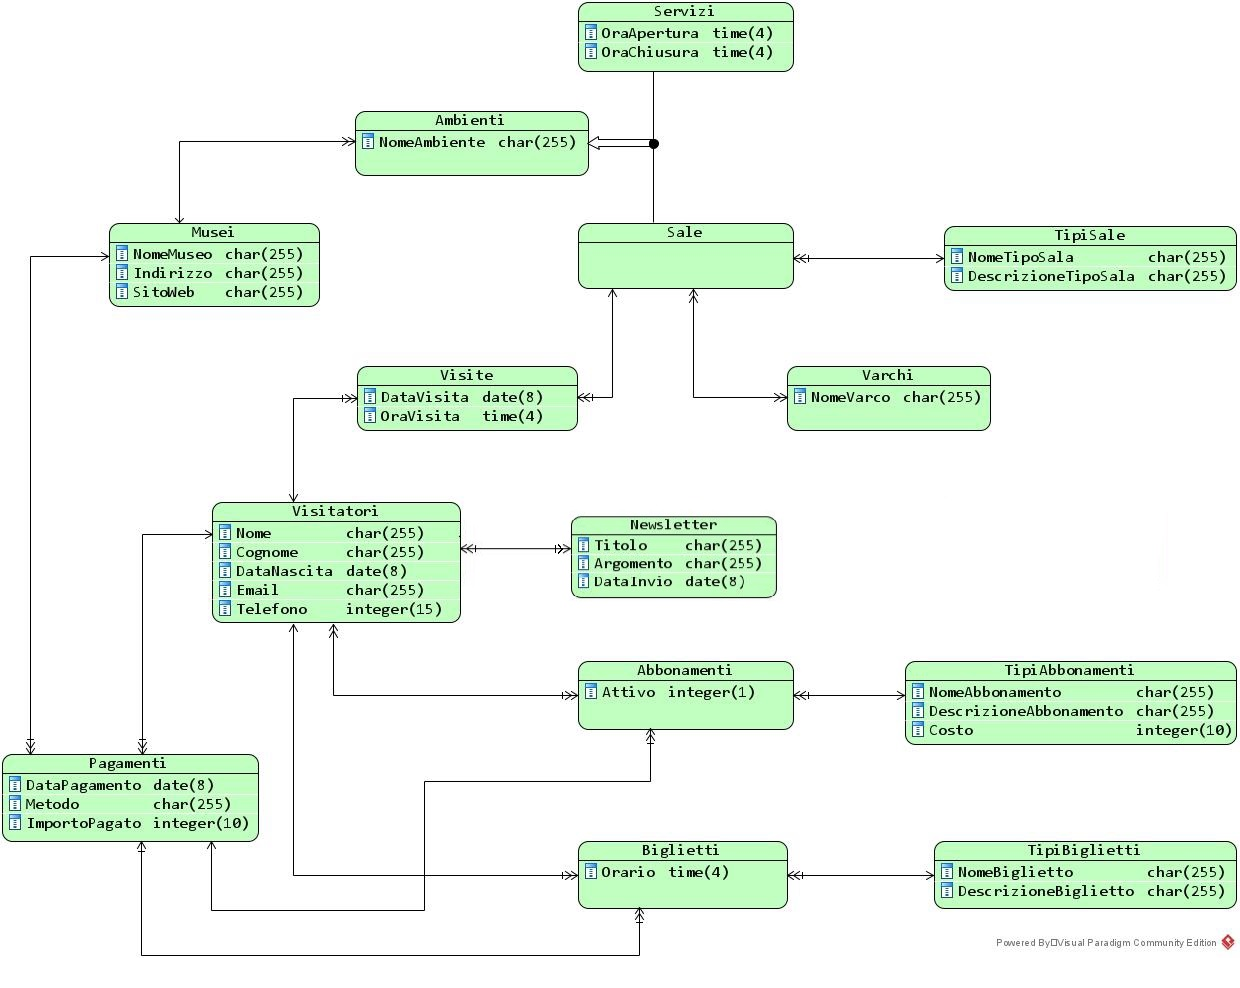
\includegraphics[width=17cm]{concettualegiusto.png}

\subsection{Vincoli}

\subsubsection{Vincoli intrarelazionali}
\begin{itemize}
    \item I seguenti attributi sono gli unici che possono assumere il valore NULL:
    \begin{itemize}
        \item \textit{Visitatori.Email}: i visitatori non sono obbligati a fornire l'indirizzo e-mail.
        \item \textit{Visitatori.Telefono}: i visitatori non sono obbligati a fornire il numero di cellulare.
    \end{itemize}
    \item \textit{Abbonamenti.Attivo} è un booleano che vale 1 se l'abbonamento in questione è attivo, 0 se è terminato.
    \item \textit{Visitatori.Telefono} non può avere meno di 9 cifre.
    \item \textit{Pagamenti.ImportoPagato} deve essere $>$ 0.
    \item \textit{TipiAbbonamenti.Costo} deve essere $>$ 0.
\end{itemize}

\subsubsection{Vincoli interrelazionali}
    \begin{itemize}
        \item In caso di visitatore con biglietto, il pagamento avviene alla fine della visita al museo. Di conseguenza la riga della tabella \textit{Pagamenti} viene riempita in un secondo momento rispetto alla riga della tabella \textit{Biglietti}. Ciò implica che la chiave esterna \textit{Biglietti.IdPagamento} è NULL fino a quando non verrà pagato il relativo biglietto.
        \item Se un visitatore acquista \textit{n} abbonamenti allora \textit{Pagamenti.ImportoPagato} deve essere $\geq$ di \textit{n} * \textit{TipiAbbonamenti.Costo} degli abbonamenti a cui si riferisce.
        \item Un visitatore può accedere alle sale esclusive sse ha un abbonamento speciale attivo.
    \end{itemize}

\section{Schema logico relazionale}

\subsection{Formato grafico}
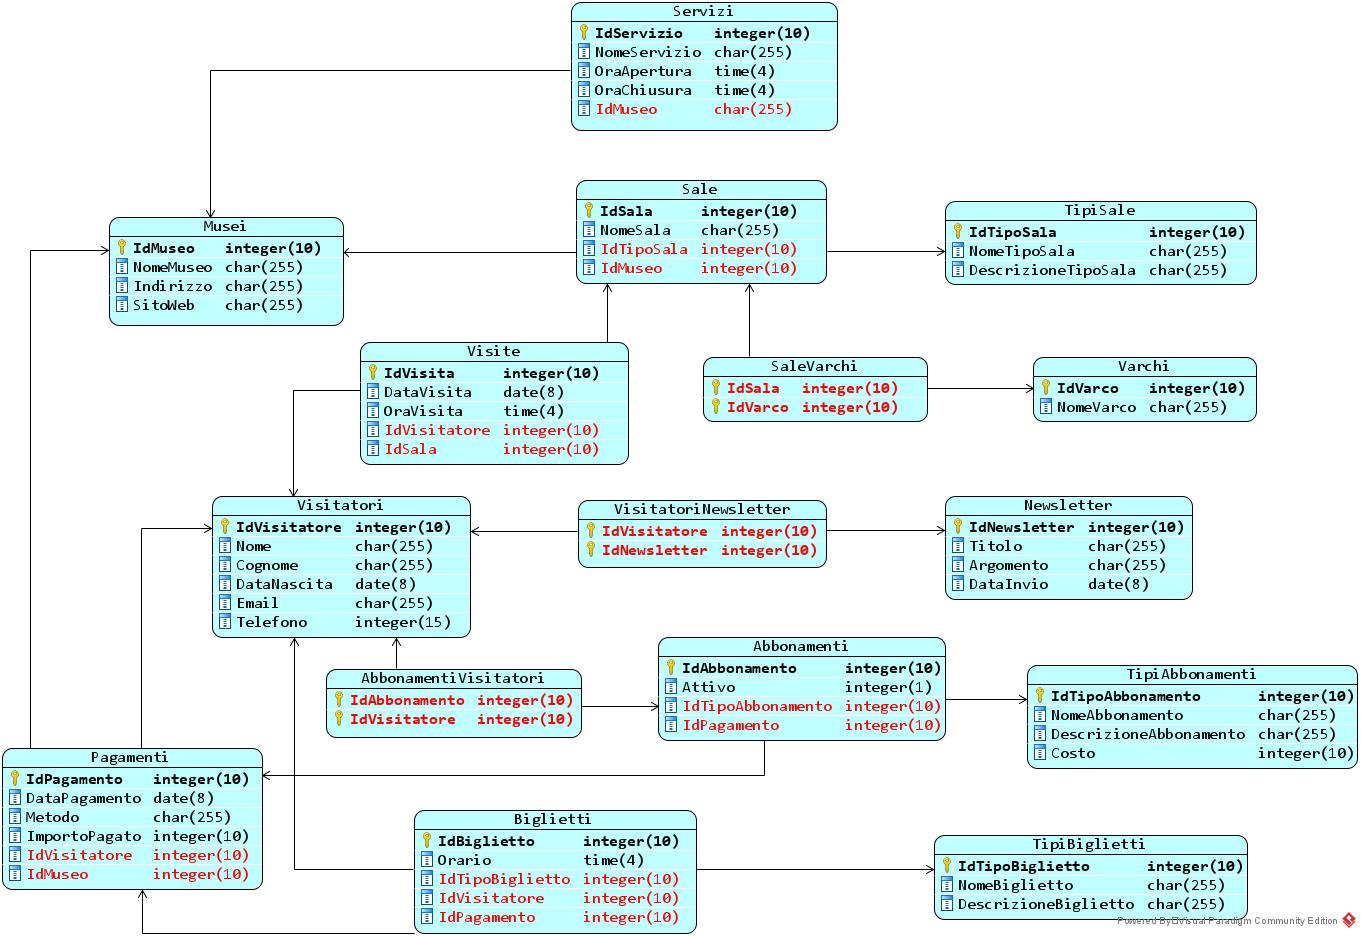
\includegraphics[width=17cm]{relazionale.jpg}

\subsection{Formato testuale}
\begin{itemize}
    \item \textbf{Musei}(\underline{IdMuseo}, NomeMuseo, Indirizzo, SitoWeb)
    \item \textbf{Servizi}(\underline{IdServizio}, NomeServizio, OraApertura, OraChiusura, IdMuseo*)
    \item \textbf{Sale}(\underline{IdSala}, NomeSala, IdTipoSala*, IdMuseo*)
    \item \textbf{TipiSale}(\underline{IdTipoSala}, NomeTipoSala, DescrizioneTipoSala)
    \item \textbf{SaleVarchi}(\underline{IdSala*, IdVarco*})
    \item \textbf{Varchi}(\underline{IdVarco}, NomeVarco)
    \item \textbf{Visite}(\underline{IdVisita}, DataVisita, OraVisita, IdVisitatore*, IdSala*)
    \item \textbf{Visitatori}(\underline{IdVisitatore}, Nome, Cognome, DataNascita, Email, Telefono)
    \item \textbf{VisitatoriNewsletter}(\underline{IdVisitatore*, IdNewsletter*})
    \item \textbf{Newsletter}(\underline{IdNewsletter}, Titolo, Argomento, DataInvio)
    \item \textbf{AbbonamentiVisitatori}(\underline{IdAbbonamento*, IdVisitatore*})
    \item \textbf{Abbonamenti}(\underline{IdAbbonamento}, Attivo, IdTipoAbbonamento*, IdPagamento*)
    \item \textbf{TipiAbbonamenti}(\underline{IdTipoAbbonamento}, NomeAbbonamento, DescrizioneAbbonamento, Costo)
    \item \textbf{Biglietti}(\underline{IdBiglietto}, Orario, IdTipoBiglietto*, IdVisitatore*, IdPagamento*)
    \item \textbf{TipiBiglietti}(\underline{IdTipoBiglietto}, NomeBiglietto, DescrizioneBiglietto)
    \item \textbf{Pagamenti}(\underline{IdPagamento}, DataPagamento, Metodo, ImportoPagato, IdVisitatore*, IdMuseo*)
\end{itemize}

\subsection{Dipendenze funzionali}
Le tabelle \textit{SaleVarchi}, \textit{VisitatoriNewsletter} e \textit{AbbonamentiVisitatori} sono in BCNF perché non hanno dipendenze non banali.
\\Le altre tabelle sono anch'esse in BCNF perché, come riportato di seguito, la parte sinistra di ogni dipendenza non banale è superchiave.
\begin{itemize}
    \item \textbf{Musei}
        \begin{itemize}
            \item IdMuseo $\rightarrow$ NomeMuseo, Indirizzo, SitoWeb
            \item SitoWeb $\rightarrow$ IdMuseo, NomeMuseo, Indirizzo
        \end{itemize}
    \item \textbf{Servizi} 
        \begin{itemize}
            \item IdServizio $\rightarrow$ NomeServizio, OraApertura, OraChiusura, IdMuseo
        \end{itemize}
    \item \textbf{Sale} 
        \begin{itemize}
            \item IdSala $\rightarrow$ NomeSala, IdTipoSala, IdMuseo
        \end{itemize}
    \item \textbf{TipiSale} 
        \begin{itemize}
            \item IdTipoSala $\rightarrow$ NomeTipoSala, DescrizioneTipoSala
        \end{itemize}
    \item \textbf{Varchi} 
        \begin{itemize}
            \item IdVarco $\rightarrow$ NomeVarco
        \end{itemize}
    \item \textbf{Visite} 
        \begin{itemize}
            \item IdVisita $\rightarrow$ DataVisita, OraVisita, IdVisitatore, IdSala
            \item DataVisita, OraVisita, IdVisitatore, IdSala $\rightarrow$ IdVisita
        \end{itemize}
    \item \textbf{Visitatori} 
        \begin{itemize}
            \item IdVisitatore $\rightarrow$ Nome, Cognome, DataNascita, Email, Telefono
            \item Email $\rightarrow$ IdVisitatore, Nome, Cognome, DataNascita, Telefono
            \item Telefono $\rightarrow$ IdVisitatore, Nome, Cognome, DataNascita, Email
        \end{itemize}
    \item \textbf{Newsletter} 
        \begin{itemize}
            \item IdNewsletter $\rightarrow$ Titolo, Argomento, DataInvio
            \item Titolo, Argomento, DataInvio $\rightarrow$ IdNewsletter
        \end{itemize}
    \item \textbf{Abbonamenti} 
        \begin{itemize}
            \item IdAbbonamento $\rightarrow$ Attivo, IdTipoAbbonamento, IdPagamento
        \end{itemize}
    \item \textbf{TipiAbbonamenti} 
        \begin{itemize}
            \item IdTipoAbbonamento $\rightarrow$ NomeAbbonamento, DescrizioneAbbonamento, Costo
        \end{itemize}
    \item \textbf{Biglietti} 
        \begin{itemize}
            \item IdBiglietto $\rightarrow$ Orario, IdTipoBiglietto, IdVisitatore, IdPagamento
            \item Orario, IdTipoBiglietto, IdVisitatore, IdPagamento $\rightarrow$ IdBiglietto
        \end{itemize}
    \item \textbf{TipiBiglietti} 
        \begin{itemize}
            \item IdTipoBiglietto $\rightarrow$ NomeBiglietto, DescrizioneBiglietto
        \end{itemize}
    \item \textbf{Pagamenti} 
        \begin{itemize}
            \item IdPagamento $\rightarrow$ DataPagamento, Metodo, ImportoPagato, IdVisitatore, IdMuseo
        \end{itemize}
\end{itemize}

\section{Interrogazioni in SQL}
\begin{center}
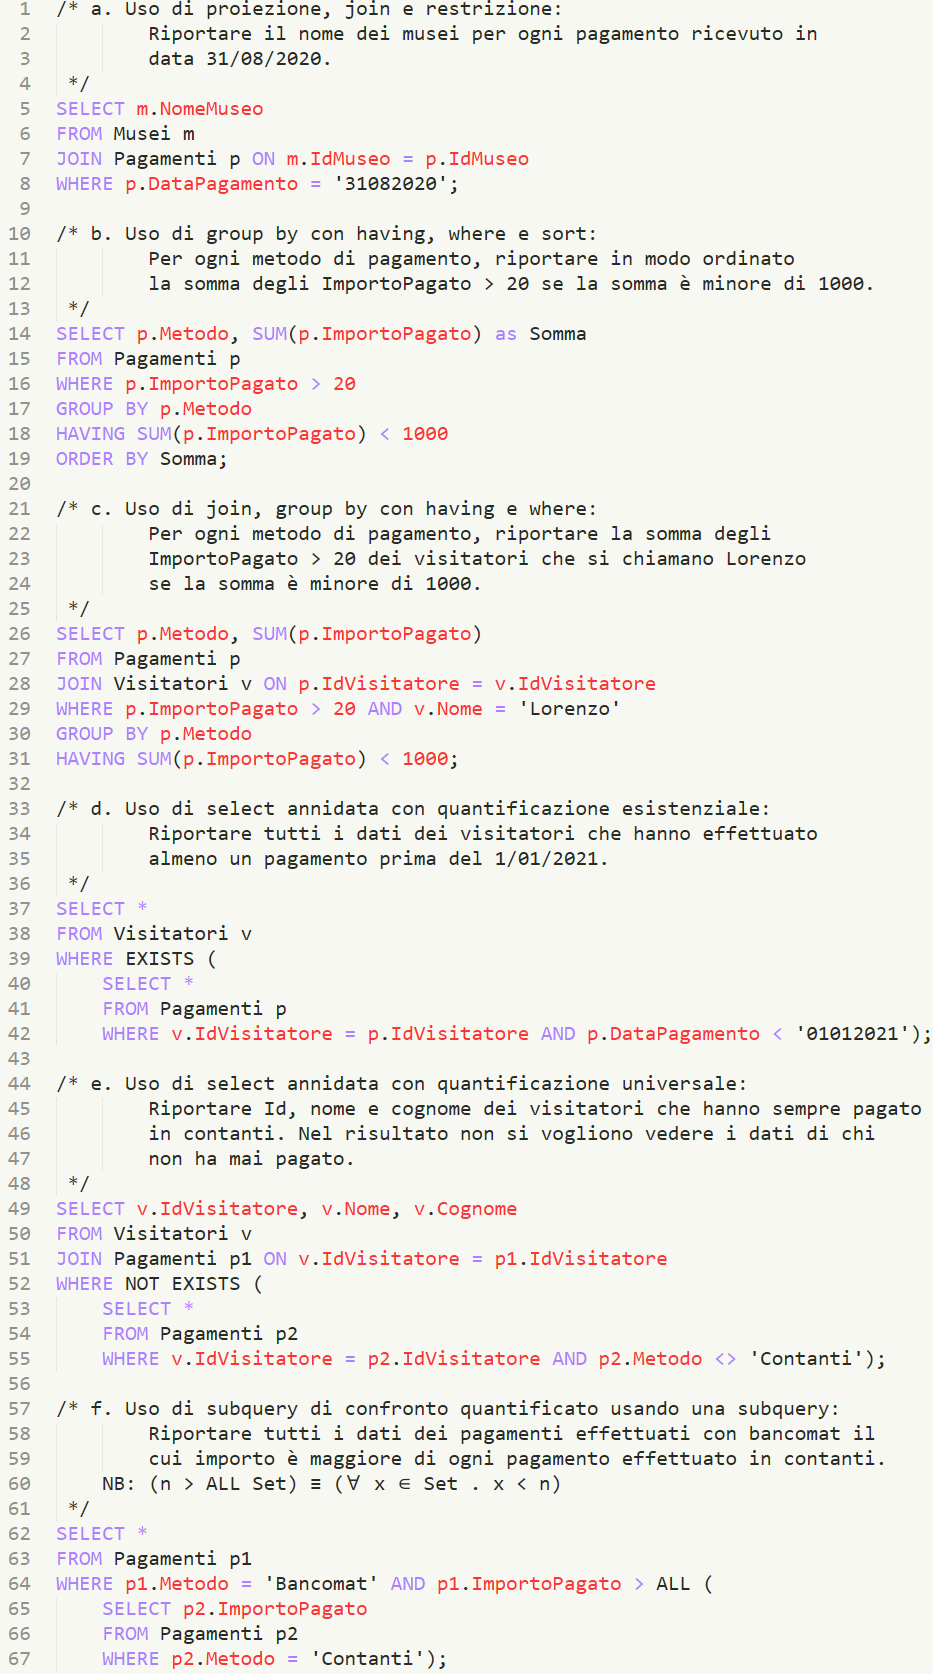
\includegraphics[width=13.3cm]{query2.png}
\end{center}

\section{Piani di accesso}

\subsection{Query (a)} 
\subsubsection{Piano di accesso logico}
\begin{center}
    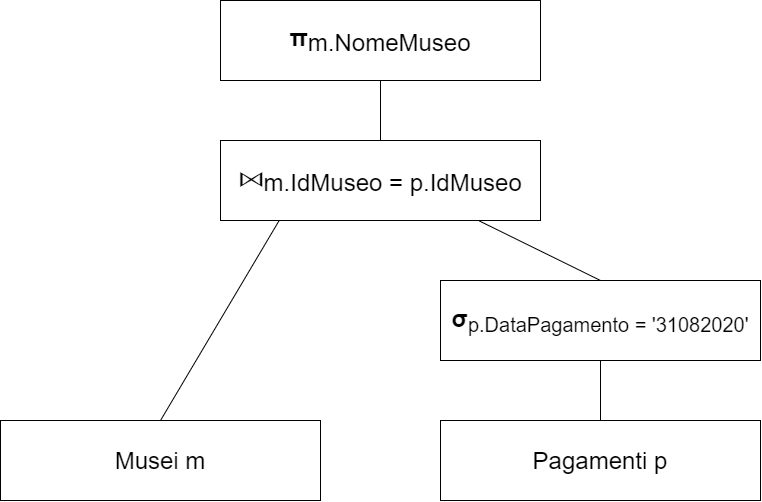
\includegraphics[width=10cm]{pianoLogicoQueryA.png}
\end{center}
\subsubsection{Piano di accesso fisico senza indici}
\begin{center}
    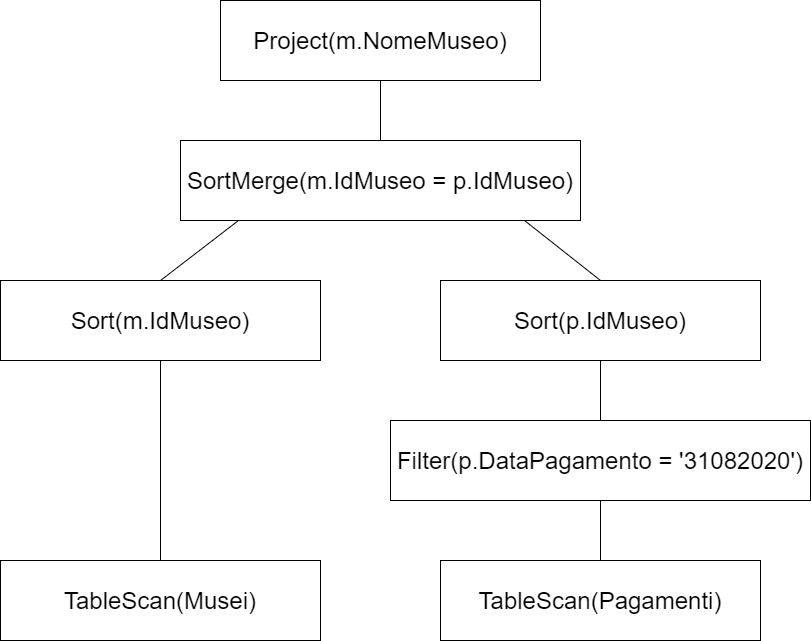
\includegraphics[width=10cm]{pianoFisicoQueryA.png}
\end{center}
\subsubsection{Piano di accesso fisico con indici}
\begin{center}
    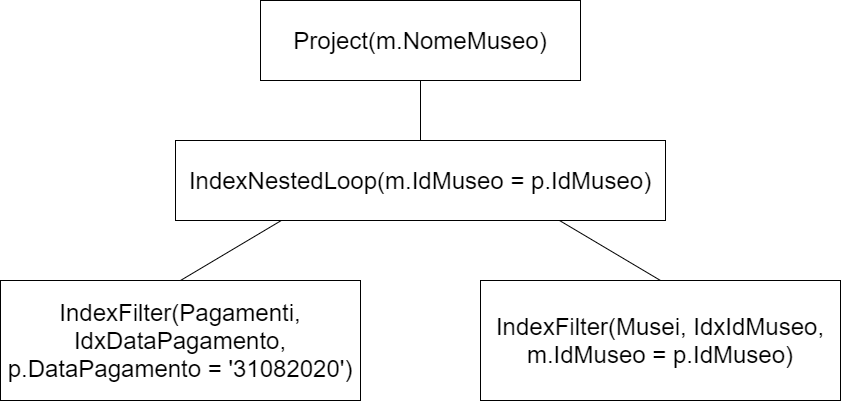
\includegraphics[width=10cm]{pianoIdxQueryA.png}
\end{center}

\subsection{Query (b)}
\subsubsection{Piano di accesso logico}
\begin{center}
    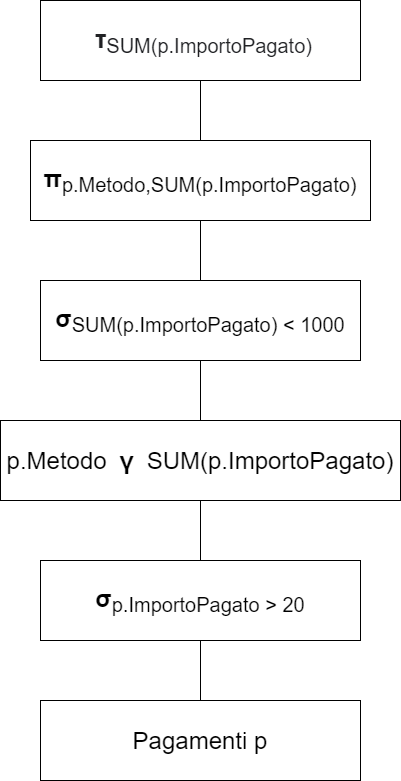
\includegraphics[width=5cm]{pianoLogicoQueryB.png}
\end{center}   
\subsubsection{Piano di accesso fisico senza indici}
\begin{center}
    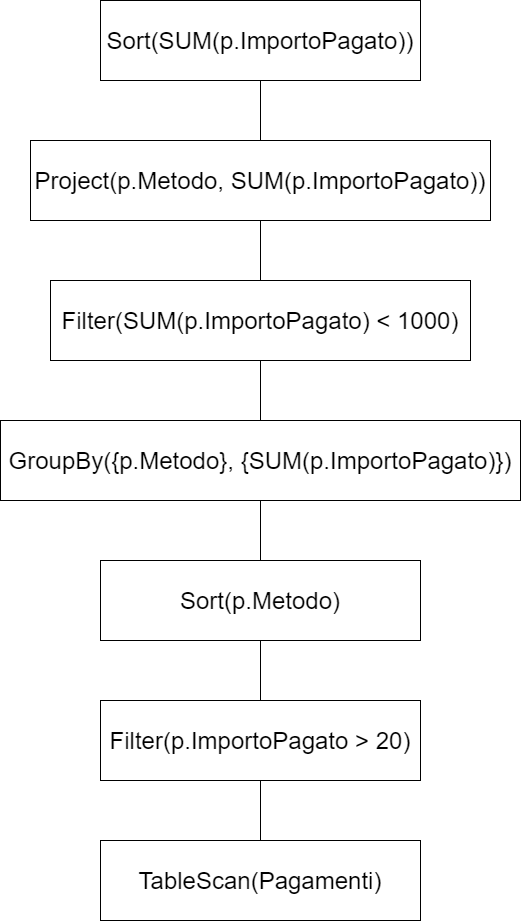
\includegraphics[width=6cm]{pianoFisicoQueryB.png}
\end{center}    
\subsubsection{Piano di accesso fisico con indici}
\begin{center}
    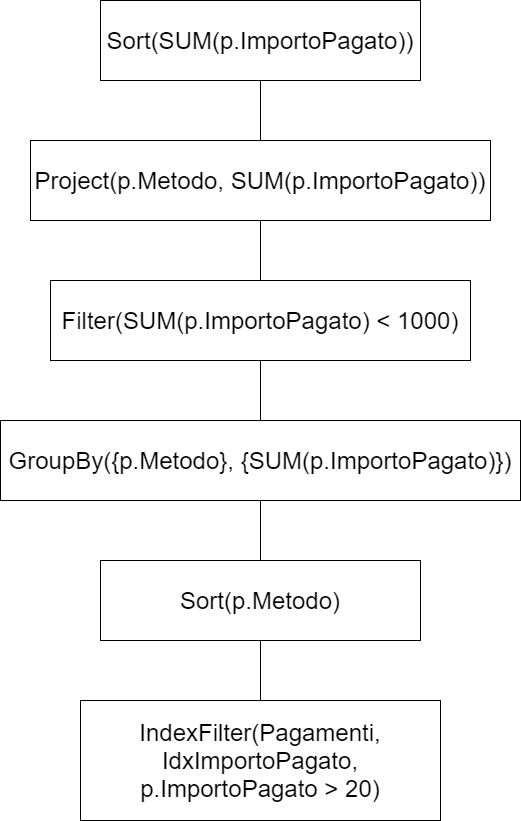
\includegraphics[width=6cm]{pianoIdxQueryB.png}
\end{center}   

\subsection{Query (c)}
\subsubsection{Piano di accesso logico}
\begin{center}
    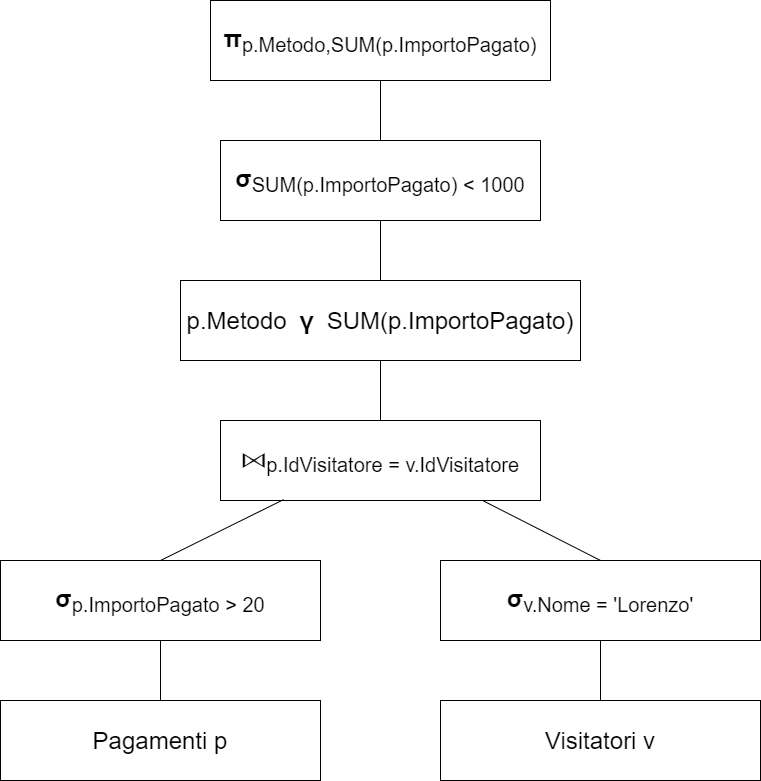
\includegraphics[width=9cm]{pianoLogicoQueryC.png}
\end{center}
\subsubsection{Piano di accesso fisico senza indici}
\begin{center}
    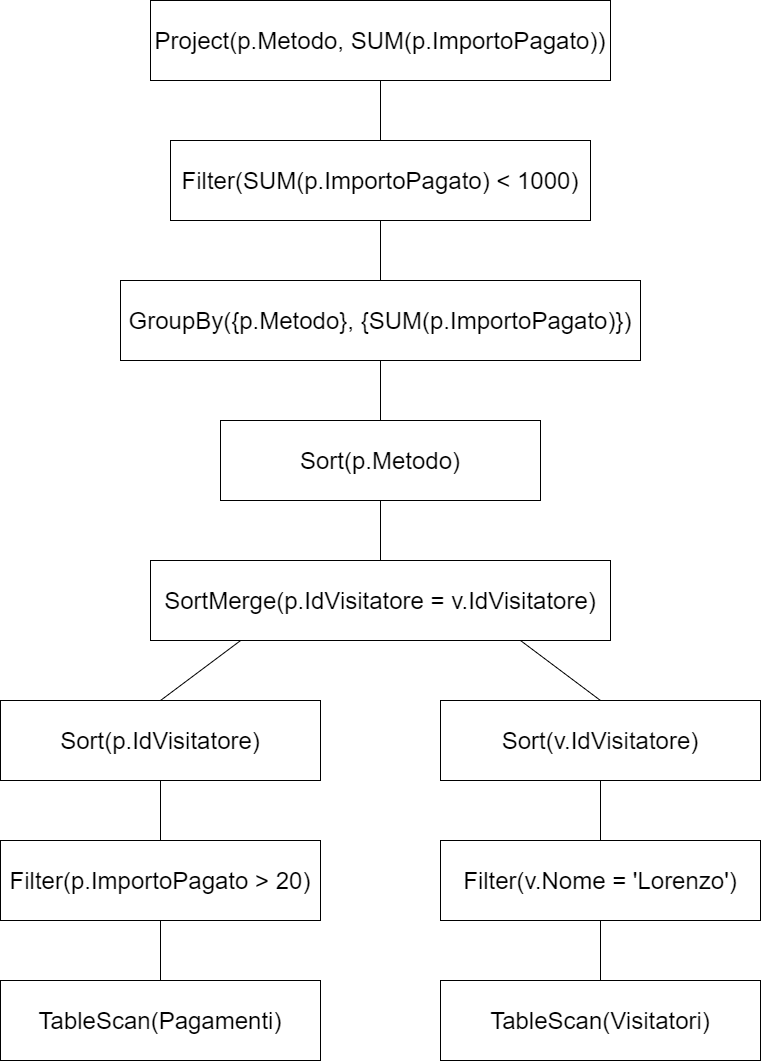
\includegraphics[width=8cm]{pianoFisicoQueryC.png}
\end{center}
\subsubsection{Piano di accesso fisico con indici}
\begin{center}
    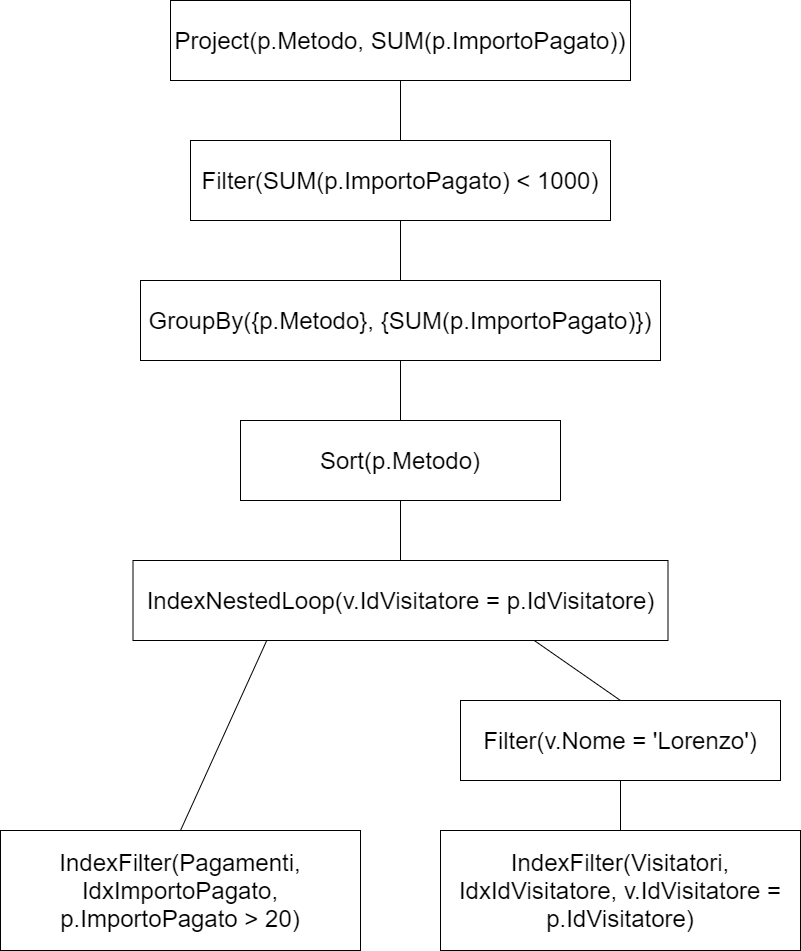
\includegraphics[width=8cm]{pianoIdxQueryC.png}
\end{center}

\end{document}




